\documentclass{uwstat518}\usepackage[]{graphicx}\usepackage[]{color}
%% maxwidth is the original width if it is less than linewidth
%% otherwise use linewidth (to make sure the graphics do not exceed the margin)
\makeatletter
\def\maxwidth{ %
  \ifdim\Gin@nat@width>\linewidth
    \linewidth
  \else
    \Gin@nat@width
  \fi
}
\makeatother

\definecolor{fgcolor}{rgb}{0.345, 0.345, 0.345}
\newcommand{\hlnum}[1]{\textcolor[rgb]{0.686,0.059,0.569}{#1}}%
\newcommand{\hlstr}[1]{\textcolor[rgb]{0.192,0.494,0.8}{#1}}%
\newcommand{\hlcom}[1]{\textcolor[rgb]{0.678,0.584,0.686}{\textit{#1}}}%
\newcommand{\hlopt}[1]{\textcolor[rgb]{0,0,0}{#1}}%
\newcommand{\hlstd}[1]{\textcolor[rgb]{0.345,0.345,0.345}{#1}}%
\newcommand{\hlkwa}[1]{\textcolor[rgb]{0.161,0.373,0.58}{\textbf{#1}}}%
\newcommand{\hlkwb}[1]{\textcolor[rgb]{0.69,0.353,0.396}{#1}}%
\newcommand{\hlkwc}[1]{\textcolor[rgb]{0.333,0.667,0.333}{#1}}%
\newcommand{\hlkwd}[1]{\textcolor[rgb]{0.737,0.353,0.396}{\textbf{#1}}}%

\usepackage{framed}
\makeatletter
\newenvironment{kframe}{%
 \def\at@end@of@kframe{}%
 \ifinner\ifhmode%
  \def\at@end@of@kframe{\end{minipage}}%
  \begin{minipage}{\columnwidth}%
 \fi\fi%
 \def\FrameCommand##1{\hskip\@totalleftmargin \hskip-\fboxsep
 \colorbox{shadecolor}{##1}\hskip-\fboxsep
     % There is no \\@totalrightmargin, so:
     \hskip-\linewidth \hskip-\@totalleftmargin \hskip\columnwidth}%
 \MakeFramed {\advance\hsize-\width
   \@totalleftmargin\z@ \linewidth\hsize
   \@setminipage}}%
 {\par\unskip\endMakeFramed%
 \at@end@of@kframe}
\makeatother

\definecolor{shadecolor}{rgb}{.97, .97, .97}
\definecolor{messagecolor}{rgb}{0, 0, 0}
\definecolor{warningcolor}{rgb}{1, 0, 1}
\definecolor{errorcolor}{rgb}{1, 0, 0}
\newenvironment{knitrout}{}{} % an empty environment to be redefined in TeX

\usepackage{alltt}
\usepackage{graphicx,amssymb,amstext,amsmath,color,verbatim, natbib,setspace}
\usepackage{natbib}
\usepackage{float}
\usepackage{wasysym}
\usepackage{subfig}
\usepackage{tikz}
%\usepackage{hyperref}
%\usepackage[all]{hypcap}
\graphicspath{{converted_graphics/}}
\usepackage{natbib}          % for author year citations \citet \citep
\bibliographystyle{plainnat} % 'plain' will be fine for many purposes
%---------------------------------------------------------
\tikzset{
  invisible/.style={opacity=0},
  visible on/.style={alt=#1{}{invisible}},
  alt/.code args={<#1>#2#3}{%
    \alt<#1>{\pgfkeysalso{#2}}{\pgfkeysalso{#3}} % \pgfkeysalso doesn't change the path
  },
}
\newcommand{\bs}{\boldsymbol}
\newcommand{\sesq}{\sigma_{\epsilon}^{2}}
\newcommand{\ssq}{\sigma^{2}}
\newcommand{\e}{\epsilon}
\newcommand{\E}{\text{E}}
\newcommand{\Var}{\text{Var}}
\newcommand{\Cov}{\text{Cov}} \newcommand{\logit}{\text{logit}}
\newcommand{\mN}{\mathcal{N}}
\newcommand{\mX}{\mathcal{X}}
         % for author year citations \citet \citep
\renewcommand{\baselinestretch}{1}
\usepackage{titling}
\setlength{\droptitle}{-1in}
\usepackage{url}
\IfFileExists{upquote.sty}{\usepackage{upquote}}{}
\begin{document}
\title{A tutorial on conducting portfolio optimization}
\author{Kirk Li}
\maketitle
\section{source scripts, load data, set parameter values}
\begin{knitrout}
\definecolor{shadecolor}{rgb}{0.969, 0.969, 0.969}\color{fgcolor}\begin{kframe}
\begin{alltt}
\hlcom{# global chunk options}
\hlkwd{library}(knitr)
opts_chunk$\hlkwd{set}(cache = TRUE, tidy = FALSE, autodep = TRUE, fig.width = 8, fig.height = 6)
\end{alltt}
\end{kframe}
\end{knitrout}


\begin{knitrout}
\definecolor{shadecolor}{rgb}{0.969, 0.969, 0.969}\color{fgcolor}\begin{kframe}
\begin{alltt}
inslib <- \hlkwd{function}(x)\{
	x <-\hlkwd{as.character}(\hlkwd{substitute}(x))
	\hlkwd{if}(!x %in% \hlkwd{rownames}(\hlkwd{installed.packages}())) 
	\{\hlkwd{install.packages}(x)\}
	\hlkwd{eval}(\hlkwd{parse}(text=\hlkwd{paste}(\hlstr{"\hlkwd{library}("},x,\hlstr{")"},sep=\hlstr{""})))\}
\hlkwd{inslib}(\hlstr{"quadprog"})
\hlkwd{inslib}(\hlstr{"xts"})
\hlkwd{inslib}(\hlstr{"corpcor"})
\hlkwd{inslib}(knitr) # inslib works w/ "
\hlkwd{source}(\hlstr{"mvo.constrained.r"})
\hlkwd{source}(\hlstr{"efront.constrained.r"})
\hlkwd{source}(\hlstr{"barplot.wts.r"})
\hlkwd{load}(\hlstr{"crsp.short.Rdata"})
\hlcom{# number of stocks}
n.stocks <- 5
\hlkwd{names}(midcap.ts)
\end{alltt}
\begin{verbatim}
##  [1] "MAT"    "EMN"    "LEG"    "AAPL"   "UTR"    "HB"     "BNK"   
##  [8] "APA"    "LNCR"   "BMET"   "DBD"    "FAST"   "AF"     "CPWR"  
## [15] "EC"     "SNV"    "HSY"    "TXT"    "APCC"   "LXK"    "market"
## [22] "t90"
\end{verbatim}
\begin{alltt}
\hlkwd{names}(smallcap.ts)
\end{alltt}
\begin{verbatim}
##  [1] "MODI"   "MGF"    "MEE"    "FCEL"   "OII"    "SEB"    "RML"   
##  [8] "AEOS"   "BRC"    "CTC"    "TNL"    "IBC"    "KWD"    "TOPP"  
## [15] "RARE"   "HAR"    "BKE"    "GG"     "GYMB"   "KRON"   "market"
## [22] "t90"
\end{verbatim}
\begin{alltt}
\hlkwd{names}(largecap.ts)
\end{alltt}
\begin{verbatim}
##  [1] "AMAT"   "AMGN"   "CAT"    "DD"     "G"      "GENZ"   "GM"    
##  [8] "HON"    "KR"     "LLTC"   "MSFT"   "ORCL"   "PG"     "PHA"   
## [15] "SO"     "TXN"    "UTX"    "WM"     "WYE"    "YHOO"   "market"
## [22] "t90"
\end{verbatim}
\begin{alltt}
returns.ts = midcap.ts[,1:n.stocks]
returns = \hlkwd{coredata}(midcap.ts[,1:n.stocks])
sum=1
mu.target=0.02 
w.initial=\hlkwd{rep}(1/n.stocks,n.stocks) 
toc=0.3
upper=\hlkwd{rep}(0.5,n.stocks)
lower=\hlkwd{rep}(-0.5,n.stocks)
group=\hlkwd{c}(\hlkwd{sample}(1:2,n.stocks,replace=T))
upper.group=\hlkwd{c}(0.5,0.5)
lower.group=\hlkwd{c}(-0.5,-0.5)
ptc=0.001
digits=4
wts.only=T
mu.min = NULL 
mu.max = NULL 
rf = .003
npoints = 20
wts.plot = T 
printout = F
bar.ylim = \hlkwd{c}(-1,4)
\hlcom{# constraint list}
\hlcom{#"sum" }
\hlcom{#"lo"}
\hlcom{#"box"}
\hlcom{#"groups"}
\hlcom{#"mu.target"}
\hlcom{#"turnover"}
\hlcom{#"turnover.doug"}
\hlcom{#"propcost"}
\end{alltt}
\end{kframe}
\end{knitrout}



Intial parameter values on constraints:
\begin{knitrout}
\definecolor{shadecolor}{rgb}{0.969, 0.969, 0.969}\color{fgcolor}\begin{kframe}
\begin{alltt}
list.arg <- \hlkwd{list}(
		sum=sum,
		mu.target=mu.target, 
		group=group, 
		upper.group=upper.group,
		lower.group=lower.group, 
		upper=upper, 
		lower=lower, 
		toc=toc, 
		w.initial=w.initial,
		ptc=ptc)	
list.arg
\end{alltt}
\begin{verbatim}
## $sum
## [1] 1
## 
## $mu.target
## [1] 0.02
## 
## $group
## [1] 2 1 1 1 2
## 
## $upper.group
## [1] 0.5 0.5
## 
## $lower.group
## [1] -0.5 -0.5
## 
## $upper
## [1] 0.5 0.5 0.5 0.5 0.5
## 
## $lower
## [1] -0.5 -0.5 -0.5 -0.5 -0.5
## 
## $toc
## [1] 0.3
## 
## $w.initial
## [1] 0.2 0.2 0.2 0.2 0.2
## 
## $ptc
## [1] 0.001
\end{verbatim}
\end{kframe}
\end{knitrout}

\newpage
\section{Null constraint}
\begin{knitrout}
\definecolor{shadecolor}{rgb}{0.969, 0.969, 0.969}\color{fgcolor}\begin{kframe}
\begin{alltt}
\hlcom{# scenario 0}
cset=NULL \hlcom{# gmv}
\hlcom{#wt plot using MU on horizontal }
\hlkwd{efrontPlot}(returns, cset, rf = .003, npoints = 20,wts.plot = T,
		bar.ylim = \hlkwd{c}(-1,4),list.arg=list.arg, wts.xlab=\hlstr{"MU"})
\end{alltt}
\end{kframe}
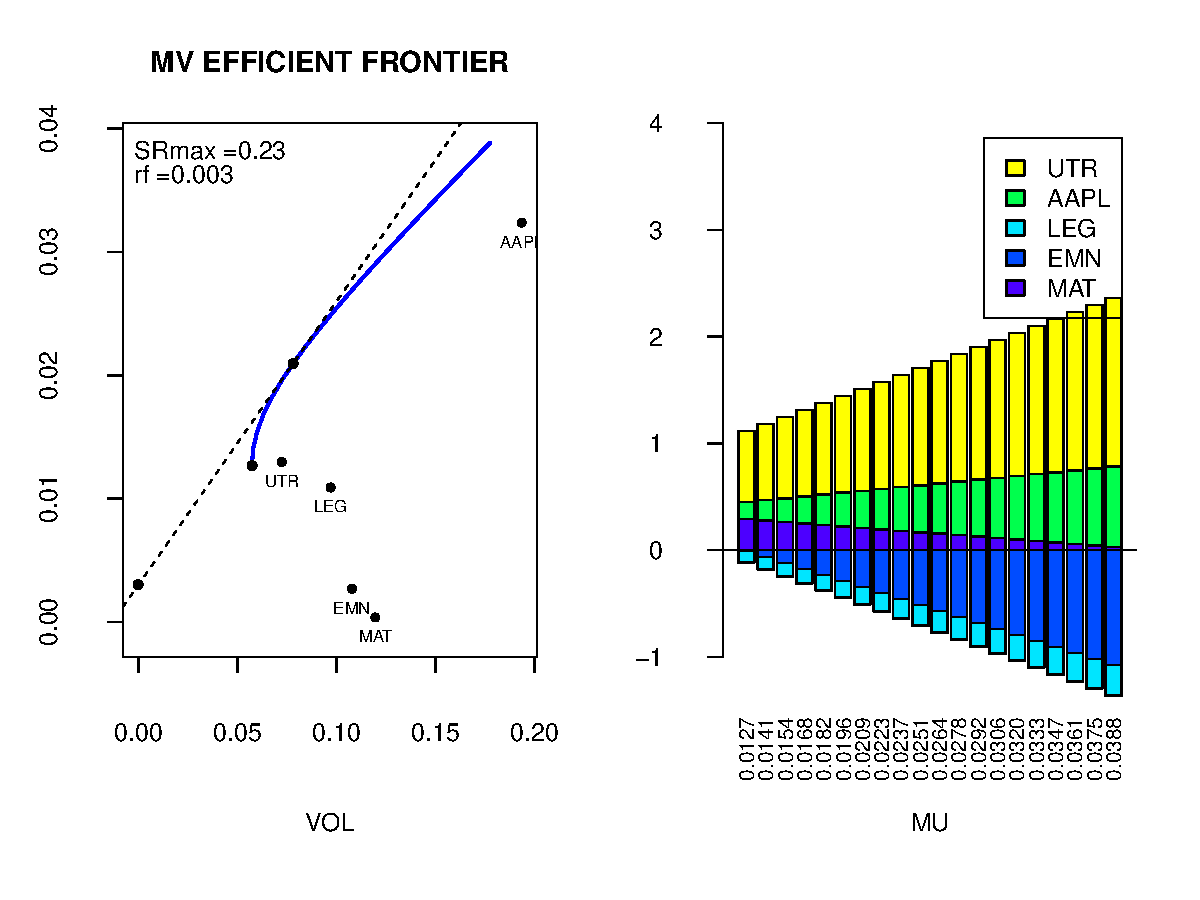
\includegraphics[width=\maxwidth]{figure/unnamed-chunk-31} 
\begin{kframe}\begin{alltt}
\hlcom{#wt plot using VOL on horizontal }
\hlkwd{efrontPlot}(returns, cset, rf = .003, npoints = 20,wts.plot = T,
		bar.ylim = \hlkwd{c}(-1,4),list.arg=list.arg, wts.xlab=\hlstr{"VOL"})
\hlkwd{mtext}(\hlkwd{paste}(clist,collapse=\hlstr{"_"}),side=1,line=3)
\end{alltt}
\end{kframe}
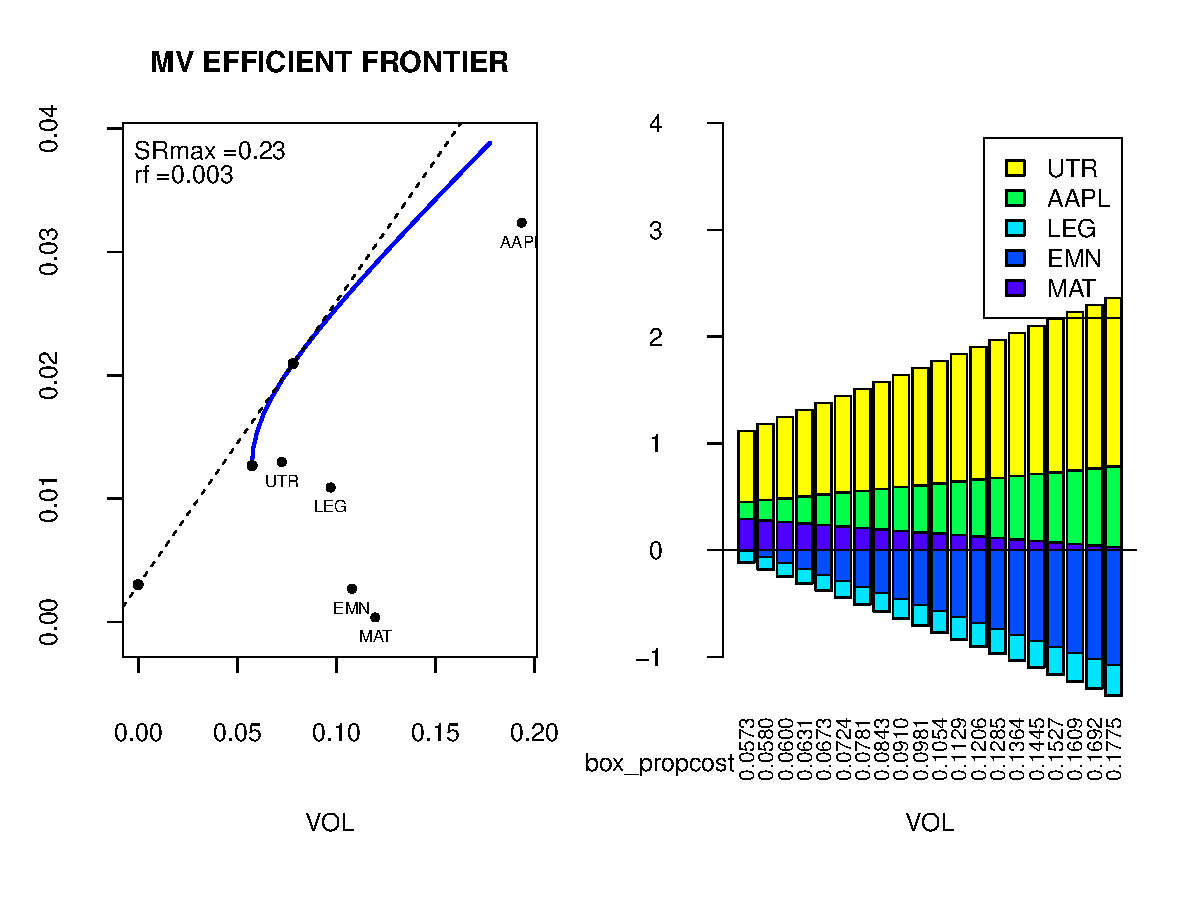
\includegraphics[width=\maxwidth]{figure/unnamed-chunk-32} 

\end{knitrout}


\section{Full investment constraint}
\begin{knitrout}
\definecolor{shadecolor}{rgb}{0.969, 0.969, 0.969}\color{fgcolor}\begin{kframe}
\begin{alltt}
\hlcom{# scenario 1}
clist <- \hlkwd{c}(\hlstr{"sum"})
cset <- NULL
cset <-\hlkwd{combine.cset}(clist=clist,returns=returns,list.arg=list.arg)
\end{alltt}
\begin{verbatim}
## sum
\end{verbatim}
\begin{alltt}
\hlkwd{gmv}(returns, cset=cset, wts.only=T,digits=4)
\end{alltt}
\begin{verbatim}
## $WTS
##     MAT     EMN     LEG    AAPL     UTR 
##  0.2917 -0.0074 -0.1076  0.1591  0.6642 
## 
## $MU.PORT
## [1] 0.0127
## 
## $SD.PORT
## [1] 0.0573
\end{verbatim}
\begin{alltt}
\hlkwd{efrontPlot}(returns, cset, rf = .003, npoints = 20,wts.plot = T,
		bar.ylim = \hlkwd{c}(-1,4),list.arg=list.arg)
\hlkwd{mtext}(\hlkwd{paste}(clist,collapse=\hlstr{"_"}),side=1,line=3)
\end{alltt}
\end{kframe}
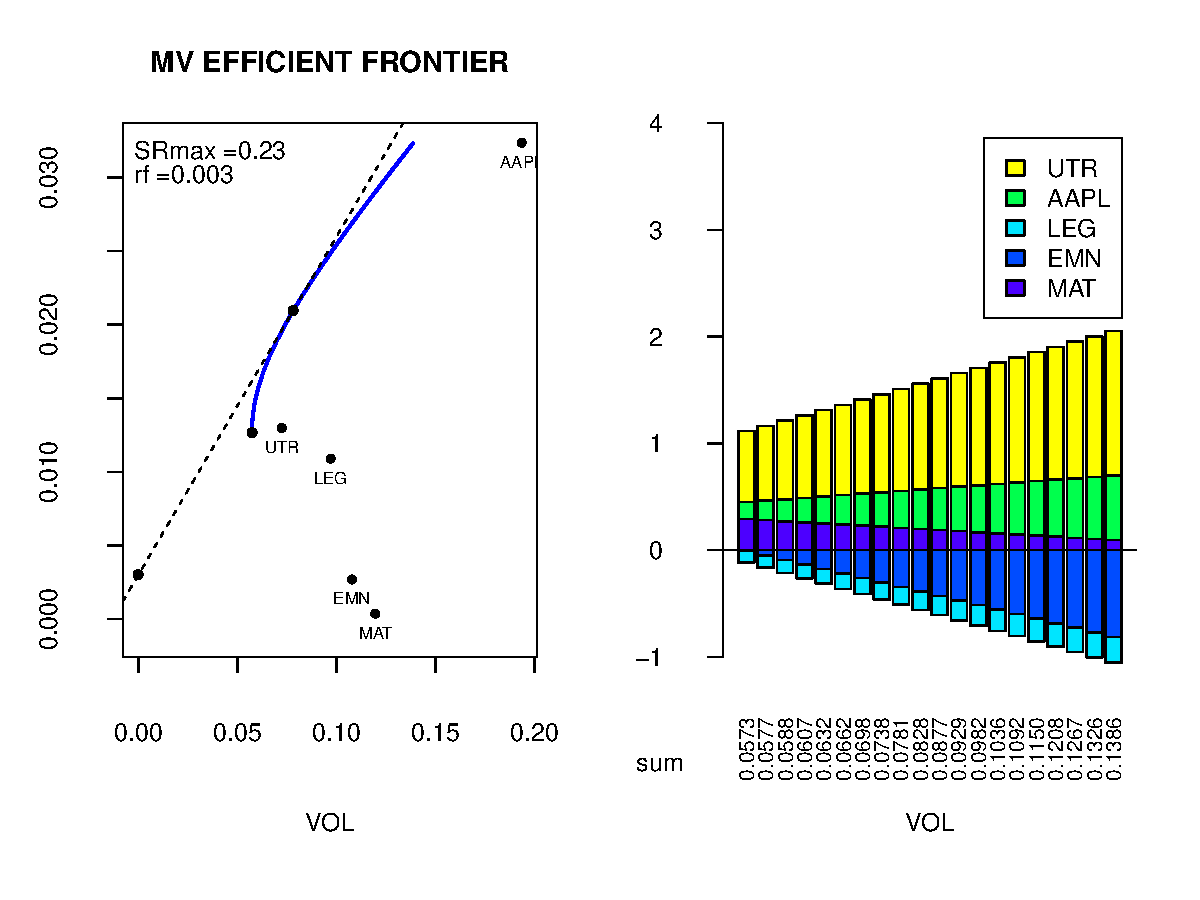
\includegraphics[width=\maxwidth]{figure/unnamed-chunk-4} 

\end{knitrout}


\section{Full investment and long only constraints}
\begin{knitrout}
\definecolor{shadecolor}{rgb}{0.969, 0.969, 0.969}\color{fgcolor}\begin{kframe}
\begin{alltt}
\hlcom{# scenario 2}
clist <- \hlkwd{c}(\hlstr{"sum"},\hlstr{"lo"})
cset <- NULL
cset <-\hlkwd{combine.cset}(clist=clist,returns=returns,list.arg=list.arg)
\end{alltt}
\begin{verbatim}
## sum 
## lo
\end{verbatim}
\begin{alltt}
\hlkwd{gmv}(returns, cset=cset, wts.only=T,digits=4)
\end{alltt}
\begin{verbatim}
## $WTS
##    MAT    EMN    LEG   AAPL    UTR 
## 0.2622 0.0000 0.0000 0.1433 0.5945 
## 
## $MU.PORT
## [1] 0.0124
## 
## $SD.PORT
## [1] 0.0578
\end{verbatim}
\begin{alltt}
\hlkwd{efrontPlot}(returns, cset, rf = .003, npoints = 20,wts.plot = T,
		bar.ylim = \hlkwd{c}(-1,4),list.arg=list.arg)
\hlkwd{mtext}(\hlkwd{paste}(clist,collapse=\hlstr{"_"}),side=1,line=3)	
\end{alltt}
\end{kframe}
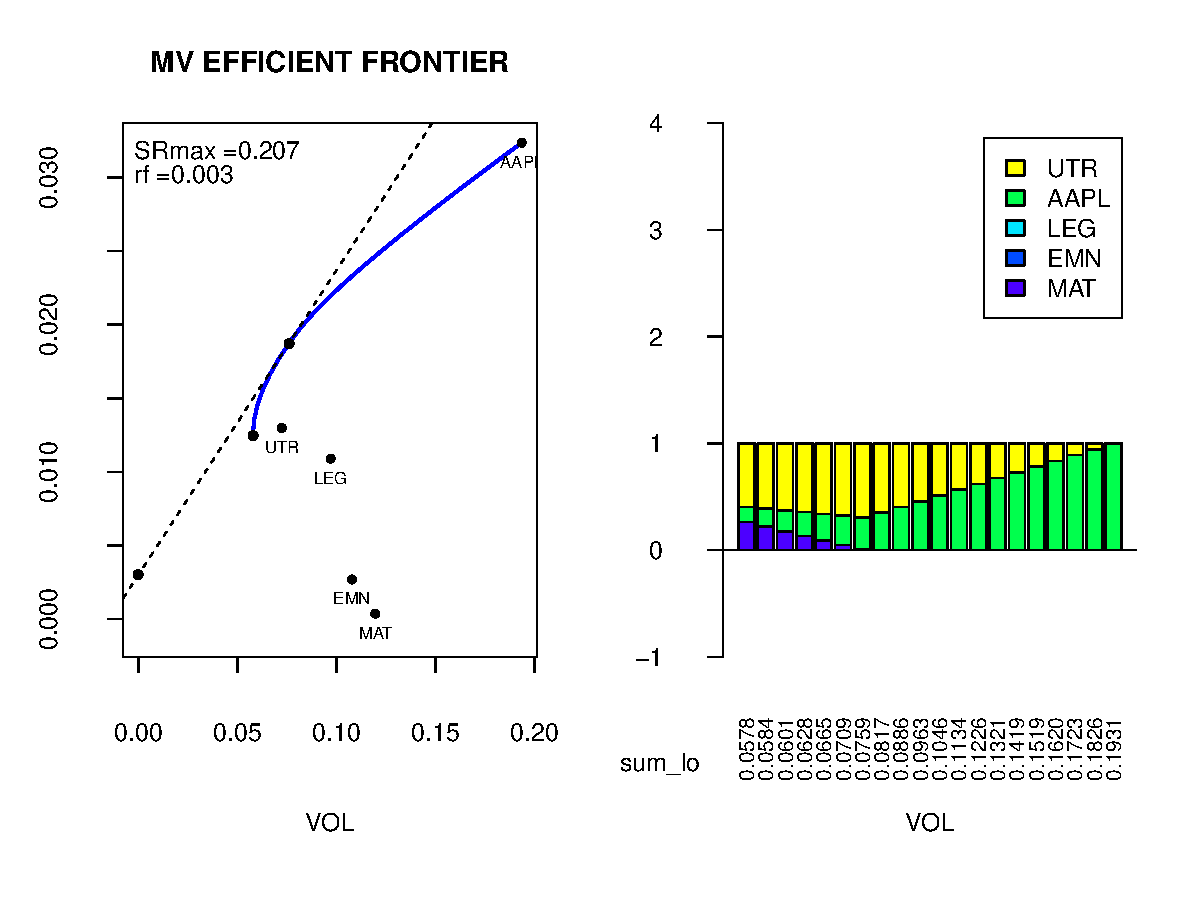
\includegraphics[width=\maxwidth]{figure/unnamed-chunk-5} 

\end{knitrout}



\section{Full investment, long only and box constraints}
\begin{knitrout}
\definecolor{shadecolor}{rgb}{0.969, 0.969, 0.969}\color{fgcolor}\begin{kframe}
\begin{alltt}
\hlcom{# scenario 3}
clist <- \hlkwd{c}(\hlstr{"sum"},\hlstr{"lo"},\hlstr{"box"})
cset <- NULL
cset <-\hlkwd{combine.cset}(clist=clist,returns=returns,list.arg=list.arg)
\end{alltt}
\begin{verbatim}
## sum 
## lo 
## box
\end{verbatim}
\begin{alltt}
\hlkwd{gmv}(returns, cset=cset, wts.only=T,digits=4)
\end{alltt}
\begin{verbatim}
## $WTS
##    MAT    EMN    LEG   AAPL    UTR 
## 0.3008 0.0372 0.0000 0.1620 0.5000 
## 
## $MU.PORT
## [1] 0.0119
## 
## $SD.PORT
## [1] 0.0585
\end{verbatim}
\begin{alltt}
\hlkwd{efrontPlot}(returns, cset, rf = .003, npoints = 20,wts.plot = T,
		bar.ylim = \hlkwd{c}(-1,4),list.arg=list.arg)
\hlkwd{mtext}(\hlkwd{paste}(clist,collapse=\hlstr{"_"}),side=1,line=3)
\end{alltt}
\end{kframe}
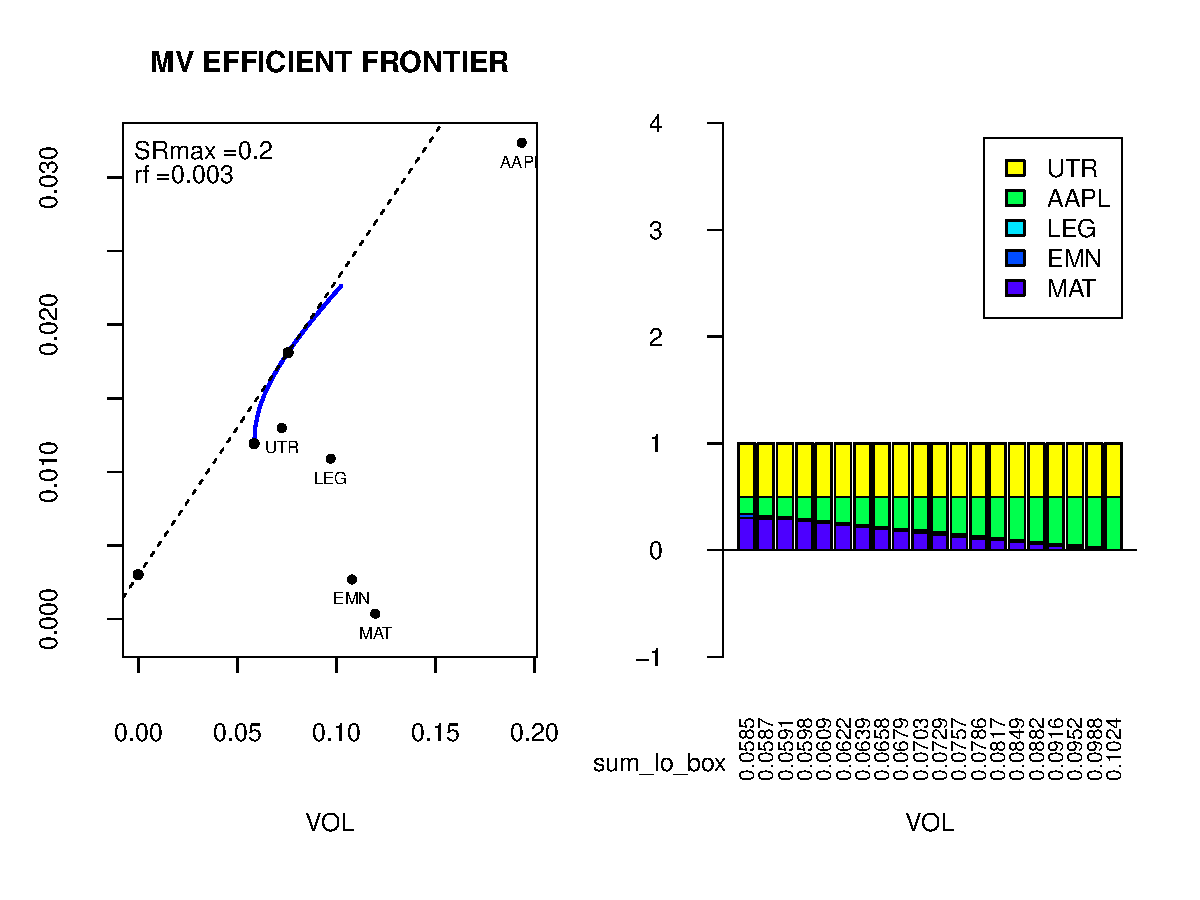
\includegraphics[width=\maxwidth]{figure/unnamed-chunk-6} 

\end{knitrout}

\newpage
\section{Full investment, long only and group constraints}
\begin{knitrout}
\definecolor{shadecolor}{rgb}{0.969, 0.969, 0.969}\color{fgcolor}\begin{kframe}
\begin{alltt}
\hlcom{# scenario 4}
clist <- \hlkwd{c}(\hlstr{"sum"},\hlstr{"lo"},\hlstr{"groups"})
cset <- NULL
cset <-\hlkwd{combine.cset}(clist=clist,returns=returns,list.arg=list.arg)
\end{alltt}
\begin{verbatim}
## sum 
## lo 
## groups
\end{verbatim}
\begin{alltt}
\hlkwd{gmv}(returns, cset=cset, wts.only=T,digits=4)
\end{alltt}
\begin{verbatim}
## $WTS
##    MAT    EMN    LEG   AAPL    UTR 
## 0.1563 0.1749 0.1845 0.1406 0.3437 
## 
## $MU.PORT
## [1] 0.0116
## 
## $SD.PORT
## [1] 0.0643
\end{verbatim}
\begin{alltt}
\hlkwd{efrontPlot}(returns, cset, rf = .003, npoints = 20,wts.plot = T,
		bar.ylim = \hlkwd{c}(-1,4),list.arg=list.arg)
\hlkwd{mtext}(\hlkwd{paste}(clist,collapse=\hlstr{"_"}),side=1,line=3)
\end{alltt}
\end{kframe}
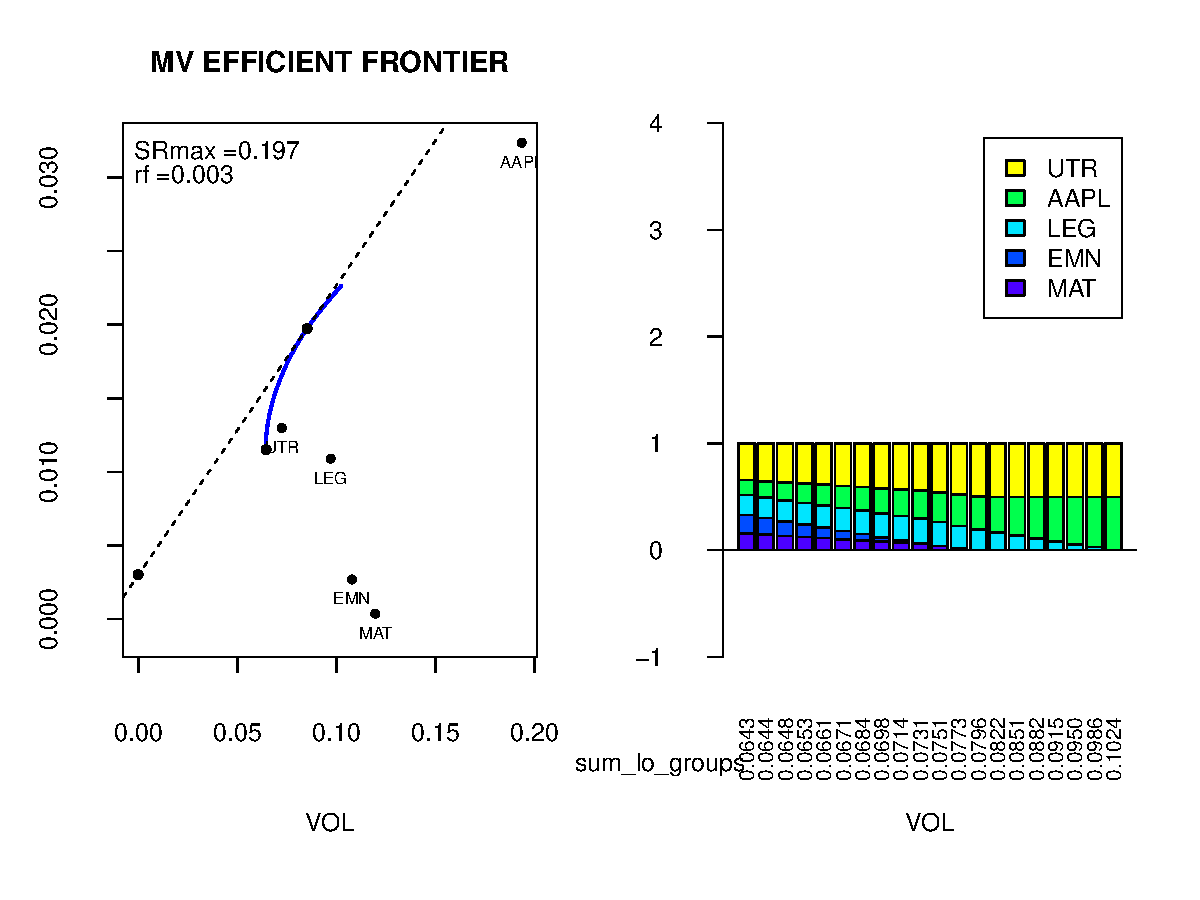
\includegraphics[width=\maxwidth]{figure/unnamed-chunk-7} 

\end{knitrout}

\newpage
\section{Full investment, long only and mean return constraints}
\begin{knitrout}
\definecolor{shadecolor}{rgb}{0.969, 0.969, 0.969}\color{fgcolor}\begin{kframe}
\begin{alltt}
\hlcom{# scenario 5}
clist <- \hlkwd{c}(\hlstr{"sum"},\hlstr{"lo"},\hlstr{"mu.target"})
cset <-\hlkwd{combine.cset}(clist=clist,returns=returns,list.arg=list.arg)
\end{alltt}
\begin{verbatim}
## sum 
## lo 
## mu.target
\end{verbatim}
\begin{alltt}
\hlkwd{gmv}(returns, cset=cset, wts.only=T,digits=4)
\end{alltt}
\begin{verbatim}
## $WTS
##    MAT    EMN    LEG   AAPL    UTR 
## 0.0000 0.0000 0.0000 0.3622 0.6378 
## 
## $MU.PORT
## [1] 0.02
## 
## $SD.PORT
## [1] 0.0831
\end{verbatim}
\end{kframe}
\end{knitrout}

\newpage
\section{Full investment, long only, box and group constraints}
\begin{knitrout}
\definecolor{shadecolor}{rgb}{0.969, 0.969, 0.969}\color{fgcolor}\begin{kframe}
\begin{alltt}
\hlcom{# scenario 6}
clist <- \hlkwd{c}(\hlstr{"sum"},\hlstr{"lo"},\hlstr{"box"},\hlstr{"groups"})
cset <- NULL
cset <-\hlkwd{combine.cset}(clist=clist,returns=returns,list.arg=list.arg)
\end{alltt}
\begin{verbatim}
## sum 
## lo 
## box 
## groups
\end{verbatim}
\begin{alltt}
\hlkwd{gmv}(returns, cset=cset, wts.only=T,digits=4)
\end{alltt}
\begin{verbatim}
## $WTS
##    MAT    EMN    LEG   AAPL    UTR 
## 0.1563 0.1749 0.1845 0.1406 0.3437 
## 
## $MU.PORT
## [1] 0.0116
## 
## $SD.PORT
## [1] 0.0643
\end{verbatim}
\begin{alltt}
\hlkwd{efrontPlot}(returns, cset, rf = .003, npoints = 20,wts.plot = T,
		bar.ylim = \hlkwd{c}(-1,4),list.arg=list.arg)
\hlkwd{mtext}(\hlkwd{paste}(clist,collapse=\hlstr{"_"}),side=1,line=3)
\end{alltt}
\end{kframe}
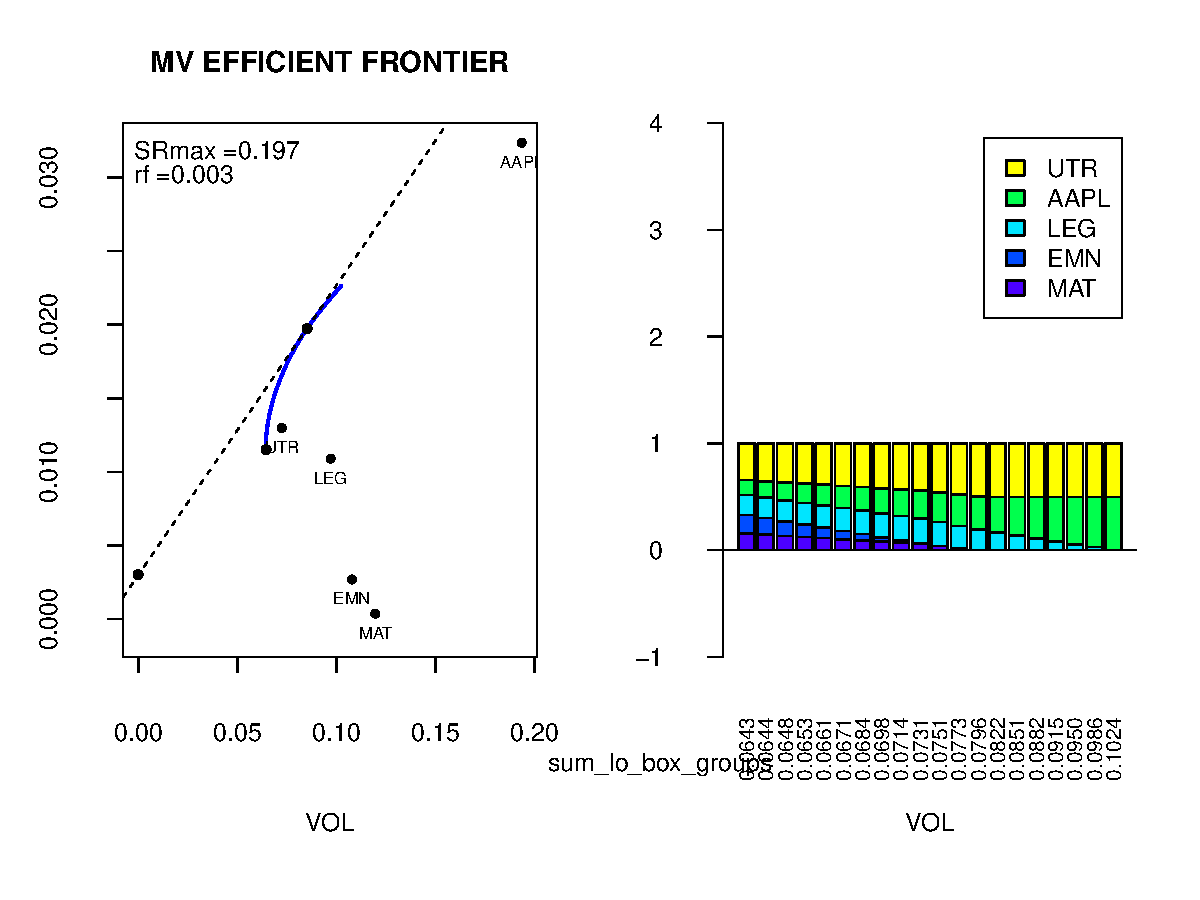
\includegraphics[width=\maxwidth]{figure/unnamed-chunk-9} 

\end{knitrout}

\newpage
\section{Full investment, long only and turnover (2 versions) constraints}
\begin{knitrout}
\definecolor{shadecolor}{rgb}{0.969, 0.969, 0.969}\color{fgcolor}\begin{kframe}
\begin{alltt}
\hlcom{# scenario 7}
clist <- \hlkwd{c}(\hlstr{"sum"},\hlstr{"lo"},\hlstr{"turnover"})
cset <- NULL
cset <-\hlkwd{combine.cset}(clist=clist,returns=returns,list.arg=list.arg)
\end{alltt}
\begin{verbatim}
## sum 
## lo 
## turnover
\end{verbatim}
\begin{alltt}
\hlkwd{gmv}(returns, cset=cset, wts.only=T,digits=4)
\end{alltt}
\begin{verbatim}
## $WTS
##    MAT    EMN    LEG   AAPL    UTR 
## 0.2000 0.1477 0.1544 0.1479 0.3500 
## 
## $MU.PORT
## [1] 0.0115
## 
## $SD.PORT
## [1] 0.063
\end{verbatim}
\begin{alltt}
\hlkwd{efrontPlot}(returns, cset, rf = .003, npoints = 20,wts.plot = T,
		bar.ylim = \hlkwd{c}(-1,4),list.arg=list.arg)
\end{alltt}
\begin{verbatim}
## [1] "turnover/propcost constraints reduced the max mean return in efficient frontier plot"
\end{verbatim}
\begin{alltt}
\hlkwd{mtext}(\hlkwd{paste}(clist,collapse=\hlstr{"_"}),side=1,line=3)
\end{alltt}
\end{kframe}
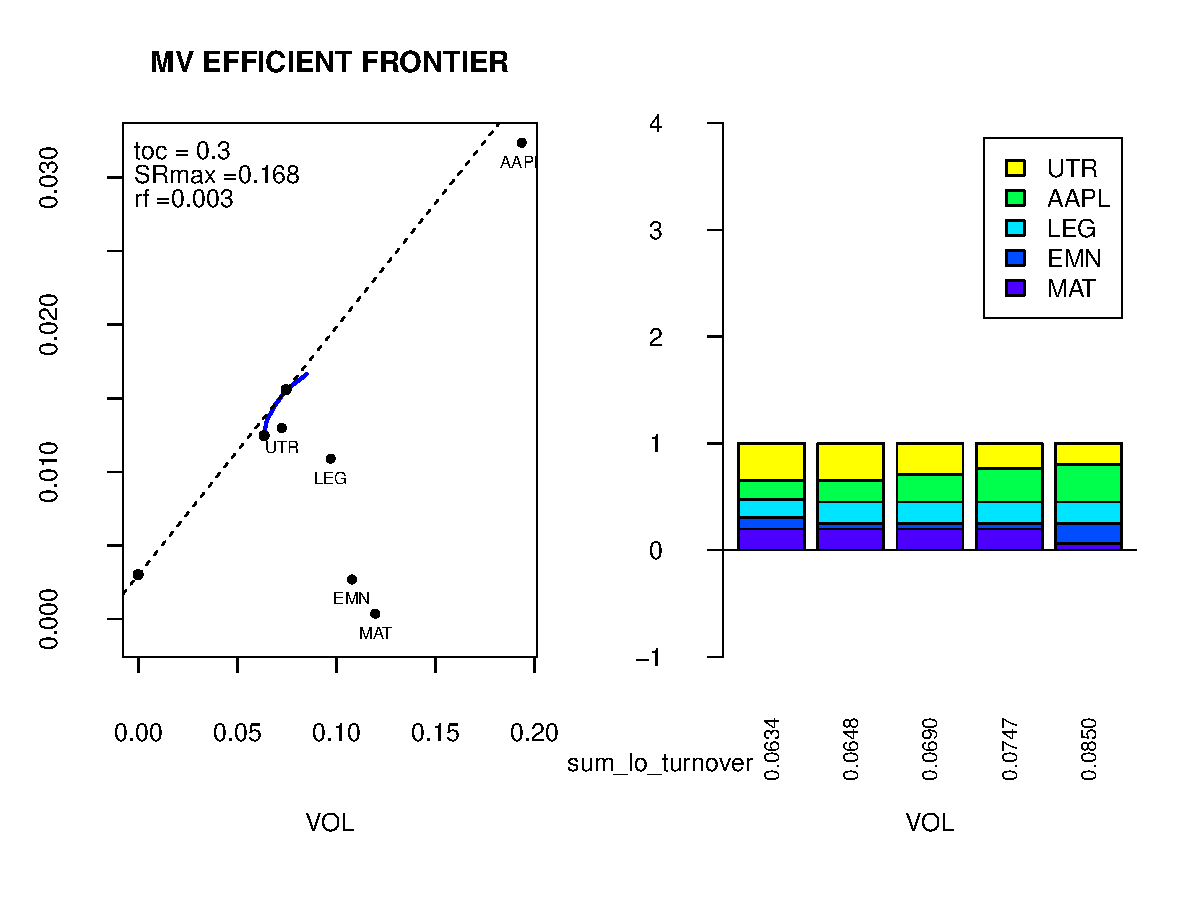
\includegraphics[width=\maxwidth]{figure/unnamed-chunk-101} 
\begin{kframe}\begin{alltt}
\hlcom{# 1+4+1+4+4+2+2+1+4+4+4  }
\hlcom{# sum+lo+mu.target+box+box+group+group+turnover+w.sell+w.buy+w.initial}

clist <- \hlkwd{c}(\hlstr{"sum"},\hlstr{"lo"},\hlstr{"turnover.doug"})
cset <- NULL
cset <-\hlkwd{combine.cset}(clist=clist,returns=returns,list.arg=list.arg)
\end{alltt}
\begin{verbatim}
## sum 
## lo 
## turnover.doug
\end{verbatim}
\begin{alltt}
\hlkwd{gmv}(returns, cset=cset, wts.only=T,digits=4)
\end{alltt}
\begin{verbatim}
## $WTS
##    MAT    EMN    LEG   AAPL    UTR 
## 0.2000 0.1477 0.1544 0.1479 0.3500 
## 
## $MU.PORT
## [1] 0.0115
## 
## $SD.PORT
## [1] 0.063
\end{verbatim}
\begin{alltt}
\hlkwd{efrontPlot}(returns, cset, rf = .003, npoints = 20,wts.plot = T,
		bar.ylim = \hlkwd{c}(-1,4),list.arg=list.arg)
\end{alltt}
\begin{verbatim}
## [1] "turnover/propcost constraints reduced the max mean return in efficient frontier plot"
\end{verbatim}
\begin{alltt}
\hlkwd{mtext}(\hlkwd{paste}(clist,collapse=\hlstr{"_"}),side=1,line=3)
\end{alltt}
\end{kframe}
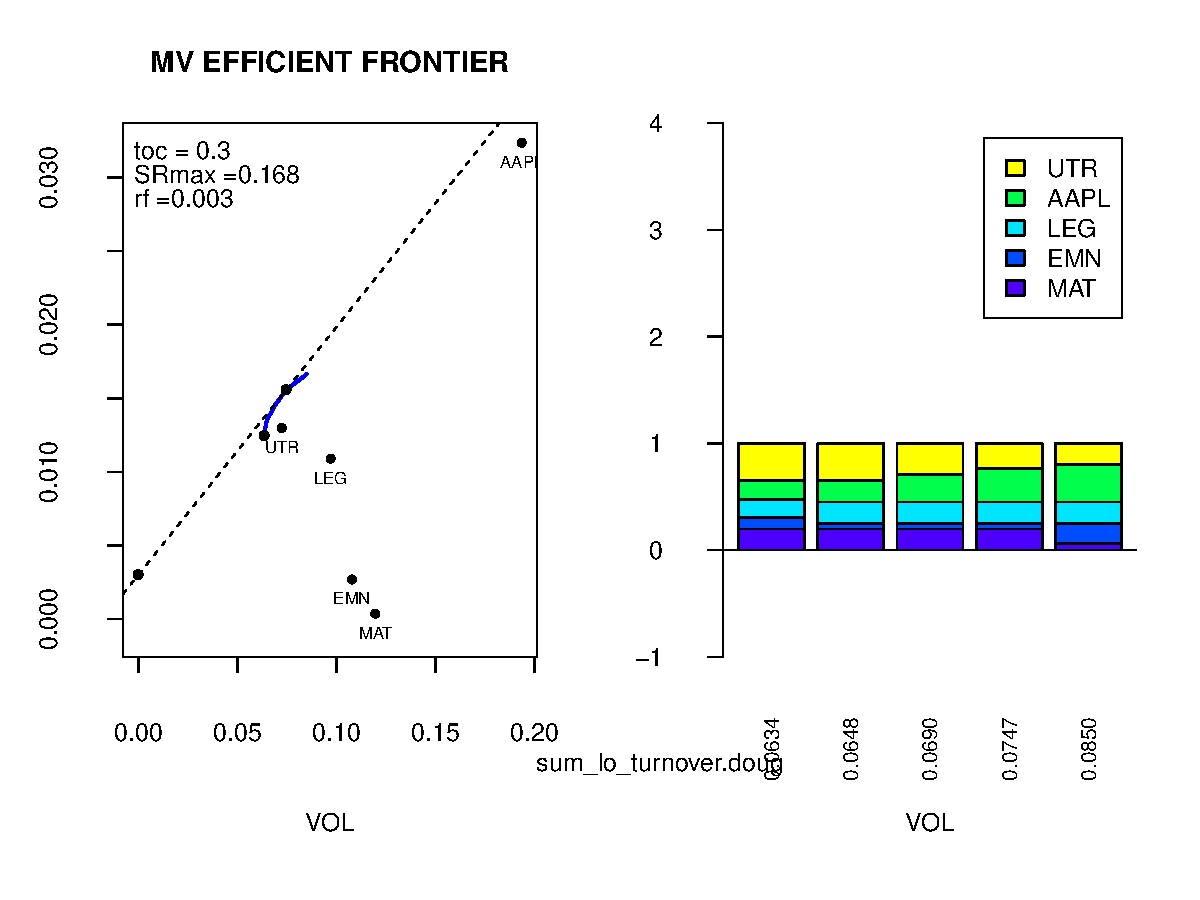
\includegraphics[width=\maxwidth]{figure/unnamed-chunk-102} 
\begin{kframe}\begin{alltt}
\hlcom{# 1+4+1+4+4+2+2+1+4+4+4  }
\hlcom{# sum+lo+mu.target+box+box+group+group+turnover+w.sell+w.buy+w.initial}
\end{alltt}
\end{kframe}
\end{knitrout}


\newpage
\section{Propcost constraints}
\begin{knitrout}
\definecolor{shadecolor}{rgb}{0.969, 0.969, 0.969}\color{fgcolor}\begin{kframe}
\begin{alltt}
\hlcom{# scenario 8 }
clist <- \hlkwd{c}(\hlstr{"propcost"})
cset <- NULL
cset <-\hlkwd{combine.cset}(clist=clist,returns=returns,list.arg)
\end{alltt}
\begin{verbatim}
## propcost
\end{verbatim}
\begin{alltt}
\hlkwd{gmv}(returns, cset=cset, wts.only=T,digits=4)
\end{alltt}
\begin{verbatim}
## $WTS
##  MAT  EMN  LEG AAPL  UTR 
##    0    0    0    0    0 
## 
## $MU.PORT
## [1] 0
## 
## $SD.PORT
## [1] 0
\end{verbatim}
\begin{alltt}

\hlkwd{efrontPlot}(returns, cset, rf = .003, npoints = 20,wts.plot = T,
		bar.ylim = \hlkwd{c}(-1,4),list.arg=list.arg)
\hlkwd{mtext}(\hlkwd{paste}(clist,collapse=\hlstr{"_"}),side=1,line=3)
\end{alltt}
\end{kframe}
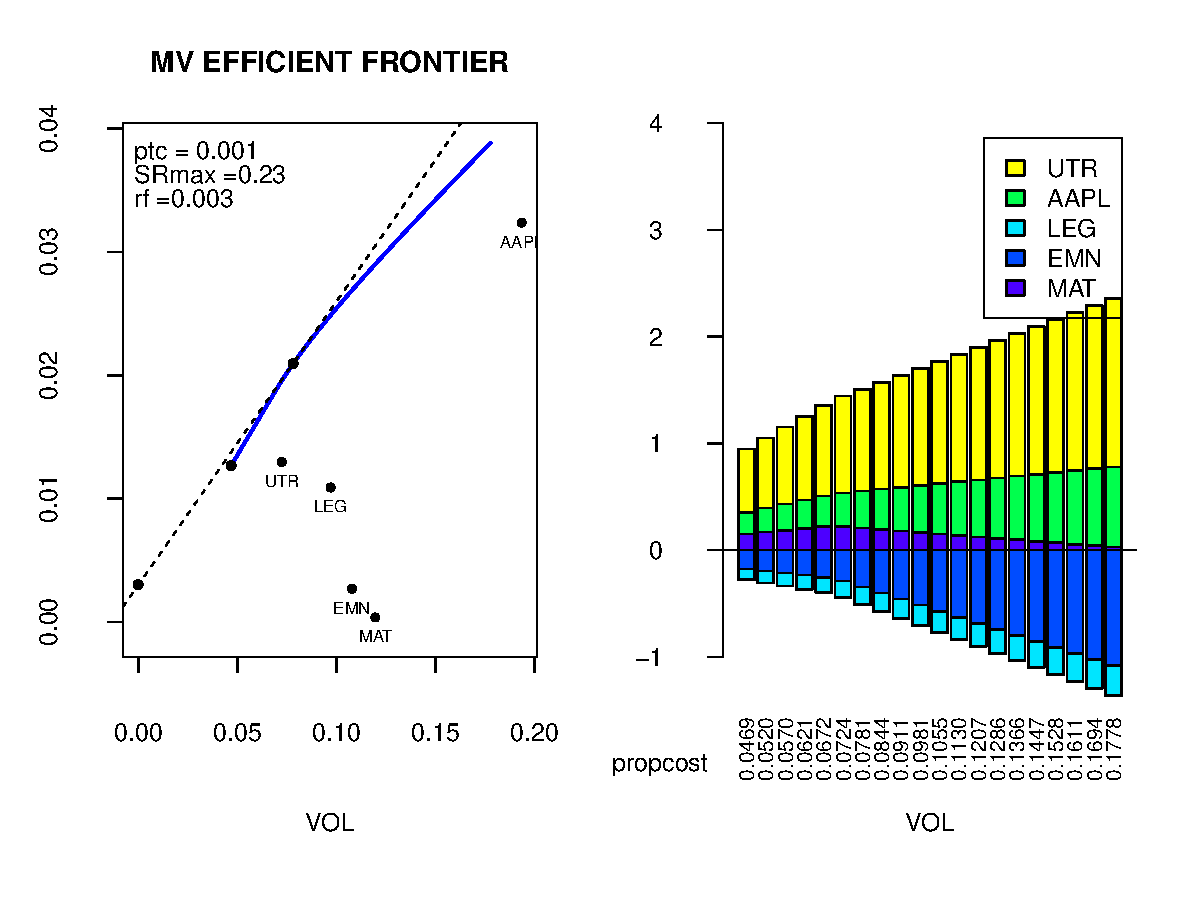
\includegraphics[width=\maxwidth]{figure/unnamed-chunk-11} 

\end{knitrout}

\newpage
\section{Long only and propcost constraints}
\begin{knitrout}
\definecolor{shadecolor}{rgb}{0.969, 0.969, 0.969}\color{fgcolor}\begin{kframe}
\begin{alltt}
\hlcom{# scenario 9 }
clist <- \hlkwd{c}(\hlstr{"lo"},\hlstr{"propcost"})
cset <- NULL
cset <-\hlkwd{combine.cset}(clist=clist,returns=returns,list.arg)
\end{alltt}
\begin{verbatim}
## lo 
## propcost
\end{verbatim}
\begin{alltt}
\hlkwd{gmv}(returns, cset=cset, wts.only=T,digits=4)
\end{alltt}
\begin{verbatim}
## $WTS
##  MAT  EMN  LEG AAPL  UTR 
##    0    0    0    0    0 
## 
## $MU.PORT
## [1] 0
## 
## $SD.PORT
## [1] 0
\end{verbatim}
\begin{alltt}

\hlkwd{efrontPlot}(returns, cset, rf = .003, npoints = 20,wts.plot = T,
		bar.ylim = \hlkwd{c}(-1,4),list.arg=list.arg)
\end{alltt}


{\ttfamily\noindent\color{warningcolor}{\#\# Warning: consider possibly relaxing constraints}}\end{kframe}
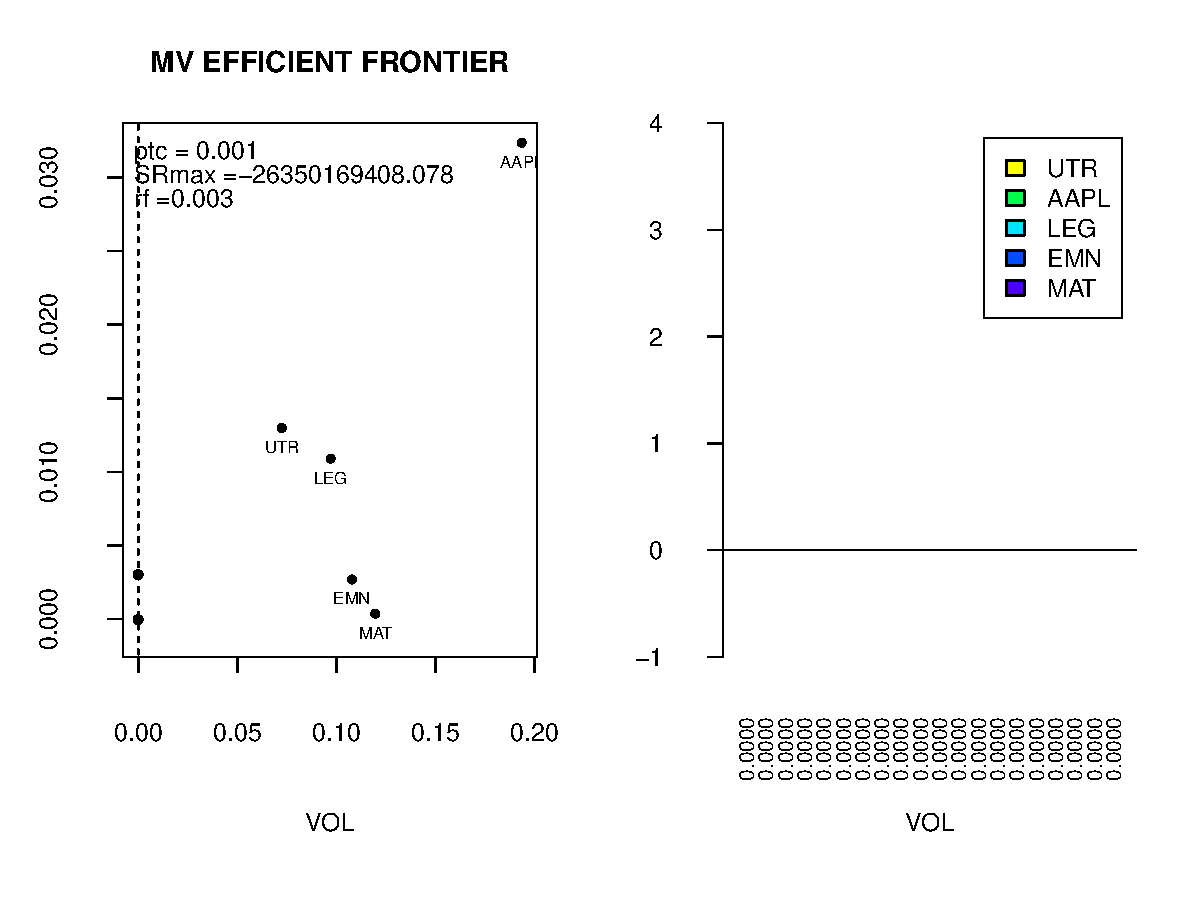
\includegraphics[width=\maxwidth]{figure/unnamed-chunk-12} 
\begin{kframe}\begin{alltt}

\hlcom{# Expected error msg: no solution, consider relaxing constraints}
\hlcom{#mtext(paste(clist,collapse="_"),side=1,line=3)}
\end{alltt}
\end{kframe}
\end{knitrout}


\newpage
\section{Box and propcost constraints}
\begin{knitrout}
\definecolor{shadecolor}{rgb}{0.969, 0.969, 0.969}\color{fgcolor}\begin{kframe}
\begin{alltt}
\hlcom{# scenario 10}
clist <- \hlkwd{c}(\hlstr{"box"},\hlstr{"propcost"})
cset <- NULL
cset <-\hlkwd{combine.cset}(clist=clist,returns=returns,list.arg)
\end{alltt}
\begin{verbatim}
## box 
## propcost
\end{verbatim}
\begin{alltt}
\hlkwd{gmv}(returns, cset=cset, wts.only=T,digits=4)
\end{alltt}
\begin{verbatim}
## $WTS
##  MAT  EMN  LEG AAPL  UTR 
##    0    0    0    0    0 
## 
## $MU.PORT
## [1] 0
## 
## $SD.PORT
## [1] 0
\end{verbatim}
\begin{alltt}

\hlkwd{efrontPlot}(returns, cset, rf = .003, npoints = 20,wts.plot = T,
		bar.ylim = \hlkwd{c}(-1,4),list.arg=list.arg)
\end{alltt}
\begin{verbatim}
## [1] "turnover/propcost constraints reduced the max mean return in efficient frontier plot"
\end{verbatim}
\begin{alltt}
\hlkwd{mtext}(\hlkwd{paste}(clist,collapse=\hlstr{"_"}),side=1,line=3)
\end{alltt}
\end{kframe}
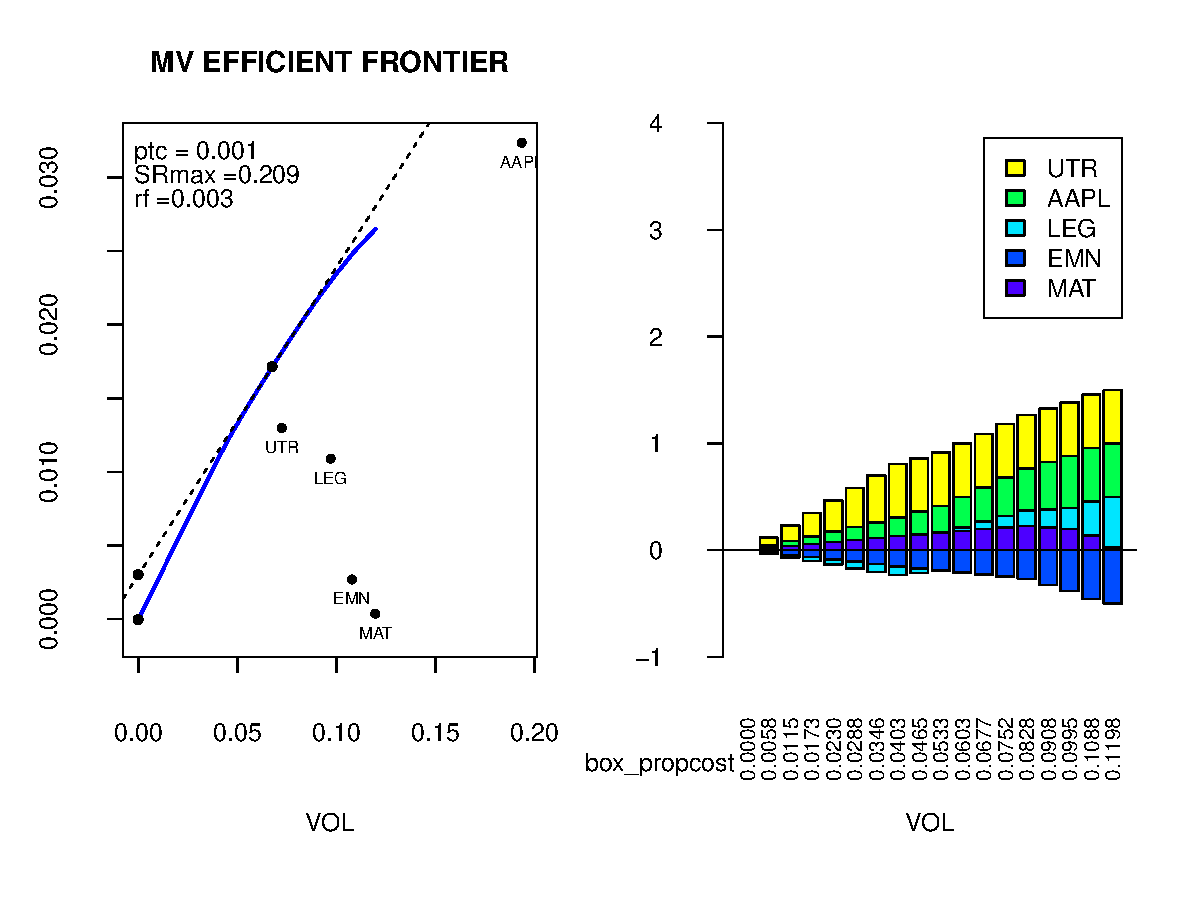
\includegraphics[width=\maxwidth]{figure/unnamed-chunk-13} 
\begin{kframe}\begin{alltt}

\hlcom{# sum constraint are not combinable with propcost constraint}
clist <- \hlkwd{c}(\hlstr{"sum"},\hlstr{"box"},\hlstr{"propcost"})
list.arg <- \hlkwd{list}( sum=sum,
                  upper=upper,
                  lower=lower,
                  ptc=ptc,
                  w.initial=w.initial)
\hlkwd{print}(list.arg)
\end{alltt}
\begin{verbatim}
## $sum
## [1] 1
## 
## $upper
## [1] 0.5 0.5 0.5 0.5 0.5
## 
## $lower
## [1] -0.5 -0.5 -0.5 -0.5 -0.5
## 
## $ptc
## [1] 0.001
## 
## $w.initial
## [1] 0.2 0.2 0.2 0.2 0.2
\end{verbatim}
\begin{alltt}
cset <- NULL
cset <-\hlkwd{combine.cset}(clist=clist,returns=returns,list.arg)
\end{alltt}
\begin{verbatim}
## sum
\end{verbatim}


{\ttfamily\noindent\bfseries\color{errorcolor}{\#\# Error: sum constraint are not combinable with propcost constraint}}\begin{alltt}
\hlcom{# Expected error msg: Error in propcost.modify(cset.i) : }
\hlcom{# sum constraint are not combinable with propcost constraint}
\end{alltt}
\end{kframe}
\end{knitrout}










\end{document}
